% Options for packages loaded elsewhere
\PassOptionsToPackage{unicode}{hyperref}
\PassOptionsToPackage{hyphens}{url}
\PassOptionsToPackage{dvipsnames,svgnames,x11names}{xcolor}
%
\documentclass[
  letterpaper,
  DIV=11,
  numbers=noendperiod]{scrartcl}

\usepackage{amsmath,amssymb}
\usepackage{iftex}
\ifPDFTeX
  \usepackage[T1]{fontenc}
  \usepackage[utf8]{inputenc}
  \usepackage{textcomp} % provide euro and other symbols
\else % if luatex or xetex
  \usepackage{unicode-math}
  \defaultfontfeatures{Scale=MatchLowercase}
  \defaultfontfeatures[\rmfamily]{Ligatures=TeX,Scale=1}
\fi
\usepackage{lmodern}
\ifPDFTeX\else  
    % xetex/luatex font selection
\fi
% Use upquote if available, for straight quotes in verbatim environments
\IfFileExists{upquote.sty}{\usepackage{upquote}}{}
\IfFileExists{microtype.sty}{% use microtype if available
  \usepackage[]{microtype}
  \UseMicrotypeSet[protrusion]{basicmath} % disable protrusion for tt fonts
}{}
\makeatletter
\@ifundefined{KOMAClassName}{% if non-KOMA class
  \IfFileExists{parskip.sty}{%
    \usepackage{parskip}
  }{% else
    \setlength{\parindent}{0pt}
    \setlength{\parskip}{6pt plus 2pt minus 1pt}}
}{% if KOMA class
  \KOMAoptions{parskip=half}}
\makeatother
\usepackage{xcolor}
\setlength{\emergencystretch}{3em} % prevent overfull lines
\setcounter{secnumdepth}{-\maxdimen} % remove section numbering
% Make \paragraph and \subparagraph free-standing
\ifx\paragraph\undefined\else
  \let\oldparagraph\paragraph
  \renewcommand{\paragraph}[1]{\oldparagraph{#1}\mbox{}}
\fi
\ifx\subparagraph\undefined\else
  \let\oldsubparagraph\subparagraph
  \renewcommand{\subparagraph}[1]{\oldsubparagraph{#1}\mbox{}}
\fi


\providecommand{\tightlist}{%
  \setlength{\itemsep}{0pt}\setlength{\parskip}{0pt}}\usepackage{longtable,booktabs,array}
\usepackage{calc} % for calculating minipage widths
% Correct order of tables after \paragraph or \subparagraph
\usepackage{etoolbox}
\makeatletter
\patchcmd\longtable{\par}{\if@noskipsec\mbox{}\fi\par}{}{}
\makeatother
% Allow footnotes in longtable head/foot
\IfFileExists{footnotehyper.sty}{\usepackage{footnotehyper}}{\usepackage{footnote}}
\makesavenoteenv{longtable}
\usepackage{graphicx}
\makeatletter
\def\maxwidth{\ifdim\Gin@nat@width>\linewidth\linewidth\else\Gin@nat@width\fi}
\def\maxheight{\ifdim\Gin@nat@height>\textheight\textheight\else\Gin@nat@height\fi}
\makeatother
% Scale images if necessary, so that they will not overflow the page
% margins by default, and it is still possible to overwrite the defaults
% using explicit options in \includegraphics[width, height, ...]{}
\setkeys{Gin}{width=\maxwidth,height=\maxheight,keepaspectratio}
% Set default figure placement to htbp
\makeatletter
\def\fps@figure{htbp}
\makeatother

\usepackage{booktabs}
\usepackage{longtable}
\usepackage{array}
\usepackage{multirow}
\usepackage{wrapfig}
\usepackage{float}
\usepackage{colortbl}
\usepackage{pdflscape}
\usepackage{tabu}
\usepackage{threeparttable}
\usepackage{threeparttablex}
\usepackage[normalem]{ulem}
\usepackage{makecell}
\usepackage{xcolor}
\KOMAoption{captions}{tableheading}
\makeatletter
\makeatother
\makeatletter
\makeatother
\makeatletter
\@ifpackageloaded{caption}{}{\usepackage{caption}}
\AtBeginDocument{%
\ifdefined\contentsname
  \renewcommand*\contentsname{Table of contents}
\else
  \newcommand\contentsname{Table of contents}
\fi
\ifdefined\listfigurename
  \renewcommand*\listfigurename{List of Figures}
\else
  \newcommand\listfigurename{List of Figures}
\fi
\ifdefined\listtablename
  \renewcommand*\listtablename{List of Tables}
\else
  \newcommand\listtablename{List of Tables}
\fi
\ifdefined\figurename
  \renewcommand*\figurename{Figure}
\else
  \newcommand\figurename{Figure}
\fi
\ifdefined\tablename
  \renewcommand*\tablename{Table}
\else
  \newcommand\tablename{Table}
\fi
}
\@ifpackageloaded{float}{}{\usepackage{float}}
\floatstyle{ruled}
\@ifundefined{c@chapter}{\newfloat{codelisting}{h}{lop}}{\newfloat{codelisting}{h}{lop}[chapter]}
\floatname{codelisting}{Listing}
\newcommand*\listoflistings{\listof{codelisting}{List of Listings}}
\makeatother
\makeatletter
\@ifpackageloaded{caption}{}{\usepackage{caption}}
\@ifpackageloaded{subcaption}{}{\usepackage{subcaption}}
\makeatother
\makeatletter
\@ifpackageloaded{tcolorbox}{}{\usepackage[skins,breakable]{tcolorbox}}
\makeatother
\makeatletter
\@ifundefined{shadecolor}{\definecolor{shadecolor}{rgb}{.97, .97, .97}}
\makeatother
\makeatletter
\makeatother
\makeatletter
\makeatother
\ifLuaTeX
  \usepackage{selnolig}  % disable illegal ligatures
\fi
\IfFileExists{bookmark.sty}{\usepackage{bookmark}}{\usepackage{hyperref}}
\IfFileExists{xurl.sty}{\usepackage{xurl}}{} % add URL line breaks if available
\urlstyle{same} % disable monospaced font for URLs
\hypersetup{
  pdftitle={Stawberries: exploratory data analysis},
  pdfauthor={MA615 TSZWAI NG},
  colorlinks=true,
  linkcolor={blue},
  filecolor={Maroon},
  citecolor={Blue},
  urlcolor={Blue},
  pdfcreator={LaTeX via pandoc}}

\title{Stawberries: exploratory data analysis}
\author{MA615 TSZWAI NG}
\date{2023-10-11}

\begin{document}
\maketitle
\ifdefined\Shaded\renewenvironment{Shaded}{\begin{tcolorbox}[breakable, boxrule=0pt, frame hidden, borderline west={3pt}{0pt}{shadecolor}, interior hidden, sharp corners, enhanced]}{\end{tcolorbox}}\fi

The data set for this assignment has been selected from:
\href{https://quickstats.nass.usda.gov}{USDA\_NASS} The data have been
stored on NASS here:
\href{https://quickstats.nass.usda.gov/results/45FBC825-B104-38E2-9802-839F5F3C7036}{USDA\_NASS\_strawb\_2023SEP19}

Make relevant observations in the document and in your code about data.
Add commentary to the code so that anthoer analysts could use or extend
your code.

Discusss missing data, inclding how you handled it. Be careful to point
out where NA's are being produced during processing and are not data
missing in the original data.

Where it is relevant, include information of how you have organized the
data for analysis. It might, for example, be helpful to know that there
is both agricultural census data and survey data. It might be helpful to
discuss data that appears to be redundant between these two sources.

Make sure you include details in your discussion and in your code about
other data and information you used in your work. Cite sources and
provide detail that would allow another analyst to reproduce your work.

\hypertarget{eda}{%
\subsection{EDA}\label{eda}}

Once the data has been cleaned and organized, you must conduct your own
EDA. Be sure to include a discussion of your analysis of the chemical
information, including citations for data and other information you have
used. Visualizations should play a key role in your analysis. Plots
should be labeled and captioned.

\hypertarget{assignment}{%
\section{Assignment}\label{assignment}}

Using our class discussions and this document as a starting point,
produce an EDA report. The report should describe the data itself so
that readers understand the data sources used in the report and how you
cleaned and organized the data for analysis.

The sections below suggest how the report might be organized. The report
should be succinct, communicating the information that you believe will
be helpful to someone doing a fuller analysis of the data or using the
data for model building. Implementation details should be included in
commentary that is included in code.

Sections of the document as it was originally presented in class have
been commented so that you can see them in the code.

\hypertarget{data-acquisition-and-assessment}{%
\subsection{Data acquisition and
assessment}\label{data-acquisition-and-assessment}}

\begin{itemize}
\tightlist
\item
  Data sources\\
\item
  Assumptions and motivations
\end{itemize}

\hypertarget{data-cleaning-and-organization}{%
\subsection{Data cleaning and
organization}\label{data-cleaning-and-organization}}

Outline the approach taked to clean and organize the data.

\begin{enumerate}
\def\labelenumi{\arabic{enumi}.}
\tightlist
\item
  Delate all the colums that only hava NA. (code by Wright, Haviland)
\end{enumerate}

\begin{enumerate}
\def\labelenumi{\arabic{enumi}.}
\setcounter{enumi}{1}
\tightlist
\item
  In the Value column, there are some data that aren't numbers, which is
  (D). They will be replaced with 0 first, then replaced by the average
  of the Value according to the type of data item they belong to. Since,
  I want to know the state and it's average value in order to graph, so
  I creat another new dataframe to show the state and it's average value
\end{enumerate}

\begin{enumerate}
\def\labelenumi{\arabic{enumi}.}
\setcounter{enumi}{2}
\tightlist
\item
  I plot a simple graph according to the data item and the average value
  they have, since the name of the data item is too long, so I do not
  specific describe which points are which data item. Also, I am
  interesting in the average value classify by the states and want to
  see which states has the highest average value.
\end{enumerate}

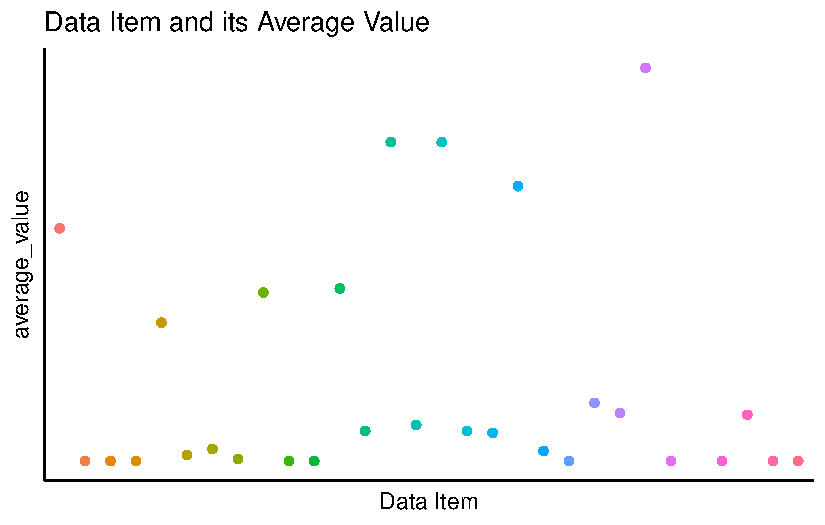
\includegraphics{USDA-NASS-data-cleaning-oct11_files/figure-pdf/unnamed-chunk-26-1.pdf}

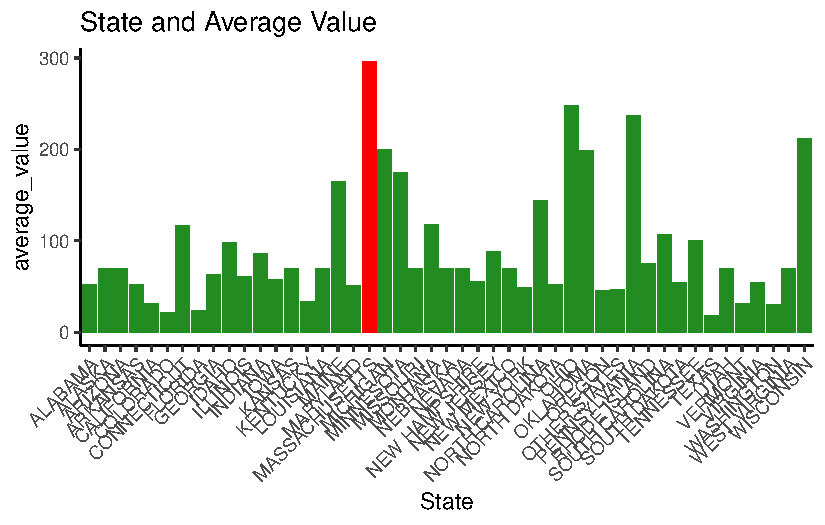
\includegraphics{USDA-NASS-data-cleaning-oct11_files/figure-pdf/unnamed-chunk-26-2.pdf}

\hypertarget{initial-questions}{%
\subsection{Initial questions}\label{initial-questions}}

\begin{itemize}
\tightlist
\item
  Initial questions about strawberries, the data, and about the work you
  are undertaking. Write these before you begin working.
\end{itemize}

I am Looking about the strawberry and it's average value according to
the state

\hypertarget{the-data}{%
\subsection{The data}\label{the-data}}

Describe the source and original condition of the data: organization,
problems with the data that needed to be addressed and so on. Cite data
sources.

The data is come from the strwb\_survey\_mkt, to look at the question I
am interested in, I need to know the average value that is classify by
the state. Since there is lots of (D) in the value, and it will occurs
error if they are not number, so I turn them into 0 and calculate out
the mean value by its state.

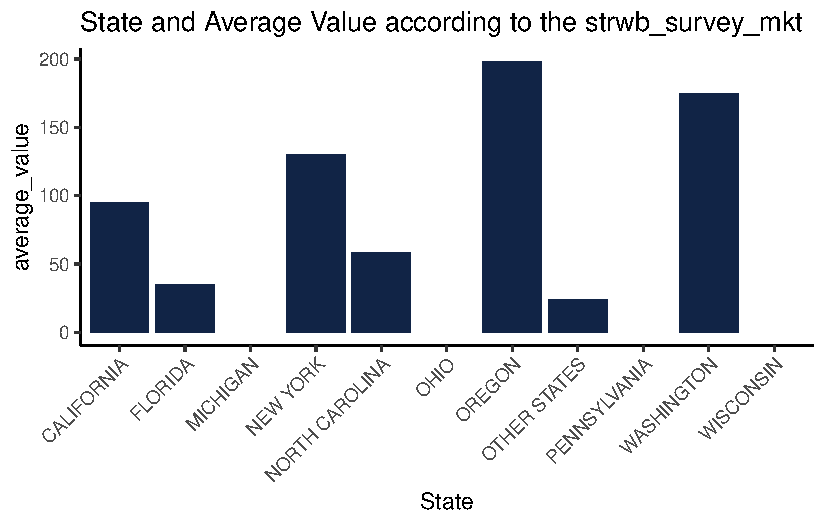
\includegraphics{USDA-NASS-data-cleaning-oct11_files/figure-pdf/unnamed-chunk-27-1.pdf}

From the graph, we can see that OREGON has the highest value. I do some
research about OREGON, and find out that OREGON has a long mild spring
and has fertile alluvial soil, that's the reason why it has the highest
strawberry value.

\hypertarget{these-references-have-been-left-in-the-document-to-help-while-you-are-writing.-cite-those-you-use-and-drop-the-rest-from-the-final-document.}{%
\subsubsection{These references have been left in the document to help
while you are writing. Cite those you use and drop the rest from the
final
document.}\label{these-references-have-been-left-in-the-document-to-help-while-you-are-writing.-cite-those-you-use-and-drop-the-rest-from-the-final-document.}}

\href{https://quickstats.nass.usda.gov/tutorials}{NASS help}

\href{https://quickstats.nass.usda.gov/src/glossary.pdf}{Quick Stats
Glossary}

\href{https://quickstats.nass.usda.gov/param_define}{Quick Stats Column
Definitions}

\href{https://www.nass.usda.gov/Statistics_by_Subject/index.php?sector=CROPS}{stats
by subject}

for EPA number lookup
\href{https://archive.epa.gov/pesticides/chemicalsearch/chemical/foia/web/html/128810.html}{epa
numbers}

\href{https://ordspub.epa.gov/ords/pesticides/f?p=APPRIL_PUBLIC:2::::::}{Active
Pesticide Product Registration Informational Listing}

pc number input
\href{https://ordspub.epa.gov/ords/pesticides/f?p=chemicalsearch:1}{pesticide
chemical search}

\href{https://comptox.epa.gov/dashboard/}{toxic chemical dashboard}

\href{https://cfpub.epa.gov/si/si_public_record_report.cfm?Lab=NCCT\&dirEntryId=209598}{ACToR
-- Aggregated Computational Toxicology Resource}

\href{https://comptox.epa.gov/dashboard/chemical/details/DTXSID0020315}{comptox
dashboard}

\href{https://pubchem.ncbi.nlm.nih.gov/}{pubChem}

The EPA PC (Pesticide Chemical) Code is a unique chemical code number
assigned by the EPA to a particular pesticide active ingredient, inert
ingredient or mixture of active ingredients.

\hypertarget{investigating-toxic-pesticides}{%
\subsection{Investigating toxic
pesticides}\label{investigating-toxic-pesticides}}

\href{https://ordspub.epa.gov/ords/pesticides/f?p=chemicalsearch:1}{start
here with chem PC code}

\href{https://ordspub.epa.gov/ords/pesticides/f?p=113:1::::RP,17,1::}{step
2} to get label (with warnings) for products using the chemical

\href{https://www.ilo.org/dyn/icsc/showcard.home}{International Chemical
safety cards}

\href{https://ordspub.epa.gov/ords/pesticides/f?p=113:1::::RP,17,1::}{Pesticide
Product and Label System}

\href{https://ordspub.epa.gov/ords/pesticides/f?p=113:17::::::}{Search
by Chemical}

\href{https://comptox.epa.gov/dashboard/}{CompTox Chemicals Dashboard}

\href{https://ordspub.epa.gov/ords/pesticides/f?p=APPRIL_PUBLIC:2::::::}{Active
Pesticide Product Registration Informational Listing}

\href{https://www.osha.gov/chemicaldata}{OSHA chemical database}

\href{http://npic.orst.edu/ingred/}{Pesticide Ingredients}

\href{http://npic.orst.edu/NPRO/}{NPIC Product Research Online (NPRO)}

\href{http://npic.orst.edu/ingred/cheminfo.html}{Databases for Chemical
Information}

\href{http://npic.orst.edu/ingred/active.html}{Pesticide Active
Ingredients}

\href{https://www.epa.gov/tsca-inventory}{TSCA Chemical Substance
Inventory}

\href{https://ordspub.epa.gov/ords/pesticides/f?p=CHEMICALSEARCH:3::::1,3,31,7,12,25:P3_XCHEMICAL_ID:2478}{glyphosate}



\end{document}
